\part{新约}


\chapter*{新约全书导论}
\addcontentsline{toc}{chapter}{新约全书导论}
“新约全书”是\UL{耶稣}死后,由其宗徒弟子,在天主圣神的默感与引导之下,所写成的经典汇集。此汇集由第二世纪起即称为《新约书》,或简称《新约》。称之为“约”,因为其中所讲论的,是天主与人类所立的盟约;称之为“新”,以别于“旧约”。“旧约”是天主与\UL{以}民在\UL{西乃}山上所立的圣约,而“新约”是\UL{基督}以自己的圣血与圣死,在天主与人间,所建立的救恩圣约(参阅\uwave{玛}26:28;\uwave{谷}14:24等处)。

“新约全书”,按圣教会古老的传授,共计二十七卷;

《历史书》五卷:《玛窦福音》、《马尔谷福音》、《路加福音》、《若望福音》和《宗徒大事录》。

《训诲书》二十一卷:圣\UL[保禄]快十四封:《罗马书》、《格林多》前后二书、《迦拉达书》、《厄弗所书》、《斐理伯书》、《哥罗森书》、《得撒洛尼》前后二书、《弟茂德》前后二书、《弟铎书》、《费肋孟书》和《希伯来书》;公函七封:《雅各伯书》、《伯多禄》前后二书、《若望》一、二、三书并《犹达书》。

《先知书》一卷:《若望默示录》。

《新约全书》,除《玛窦福音》的原文为\UL[阿刺美]文外,都是用\UL[希腊]文写成的。这些似乎有些奇怪,因为按当时\UL[耶稣]在世时,和宗徒最初讲道时所用的语言,本来都是\UL[阿刺美]语,并且全部《新约》作者,除圣\UL{路加}外,又都是\UL[犹太]人;那么为什么不用本国文字编写呢?其理由是因为只有《玛窦福音》是写给\UL[巴力斯坦]的\UL[犹太]人,而其余的书都是写给说\UL[希腊]话的基督徒,其中很少有通晓\UL[阿刺美]语的;更何况《新约》又是向天下万民所公布的;因此以当时\UL[罗马]帝国内所通行的\UL[希腊]语编写,是很自然的事。

《新约全书》(或《新经》),就宗教方面来说,远远超过《旧约全书》(或《古经》),因为天主在旧约时代只是“多次并以多种方式,藉着先知对祖先说过话”;然而在新约时代却是“藉着了对我们说了话”(\uwave{希}1:1)。如此,旧约的启示在新约内才得以圆满;旧约的预许在新约内才得以实现。所以吾人除非认识《新约》,决不能完全明了《旧约》;为此,可说《新约全书》实是世界上最重要和最宝贵的作品。


\chapter*{福音总论}
\addcontentsline{toc}{chapter}{福音总论}
“福音”一词,按其字音,原指“喜讯”;但按《新约》作者彩此词的意义来说,乃是指天主子\UL{耶稣}隆重为人,从天上给人类带来的启示,和在他完成救赎工程以后,诸宗徒向万民所宣布的得救喜讯。

这喜讯的传报,最初只靠口头的宣讲,稍后才有不少人士把\UL{耶稣}的生平与宣讲笔之于书,因而产生了“福音”的著作。按\uwave{路}1:1的记载,这样的著作在当时已为数不少,可是圣教会自初只承认《玛窦》、《马尔谷》、《路加》、《若望》这四部《福音》为受默感而写的经典,并著录在正经书目内,其他名为“福音”的著作,概著录为伪经。

“福音”书虽有四部,但所传述的“福音”却只是一个,因为四圣史所撰述的是同一的喜讯,只是在所采用形式上有所不同而已。前三部《福音》,无论是在取材和结构上,或在用字上,大致可以说相同,甚至可并列对照,一望而知彼此间所有的关系,因而有“对观福音”之称。这三部《福音》之所以如此相同,是因为前三圣史记述了大体相同的“宗徒教理讲授”:\UL[玛窦]记述了\UL[耶路撒冷]教会的传授,\UL[马尔谷]记述了\UL[罗马]教会的传授,\UL[路加]记述了\UL[安提约基雅]教会的传授。\UL[若望]因见前三《福音》已流传于世,没有重述的必要,遂由自己记忆所及,采取了一些有关的材料,在第一世纪末叶,针对当时人事环境的需要,编著了自己的《福音》,其目的是在攻击方兴的异端邪说。

四《福音》虽然不是狭义的史书,但就信实性来说:世界上没有一部史书可与之相比,因为各位作者,或是目睹所述之事的宗徒(\UL[玛窦]、\UL[若望]),或是宗徒的亲传弟子(\UL[马尔谷]、\UL[路加]),他们所依据的,全是亲历其事人物的口述;况且《福音》成书时,尚有不少耳闻目睹的证人生存于世。

四《福音》内不但包含了有关信仰绝对重要的道理,而且也给世人提示了诸德的完美模范,基督徒成全的最高理想:即为我们降生成人的天主圣子。


\chapter*{玛窦福音引言}
\addcontentsline{toc}{chapter}{玛窦福音引言}
第一部《福音》的作者是圣\UL[玛窦]宗徒。\UL[玛窦]又名\UL[肋未],是\UL[阿耳斐]的儿子(\uwave{谷}2:14)。他在\UL{耶稣}召叫之前,曾在\UL[葛法翁]作过税吏。他一被召,即刻舍弃一切,跟随了\UL{耶稣}(\uwave{玛}9:9;\uwave{谷}2:13、14;\uwave{路}5:27、28)。\UL{耶稣}升天后,他先在\UL[巴力斯坦]一带,给自己的同胞宣讲福音多年,然后动身往外方传教去了。最后死在何处何时,史无确证。圣教会从古以来,即认他为一位为主殉道的宗徒,每年九月二十一日庆祝他的瞻礼。

据最古的传授,圣教会始终认为圣\UL[玛窦]是第一部《福音》的作者;这也可由《福音》书内的暗示得到证明:例如\UL[马尔谷]与\UL[路加]记载十二位宗徒名单时,只记了\UL[玛窦]的名字,然而在第一部《福音》内,于“\UL[玛窦]”名字前却加上了受人歧视的“税吏”头衔,可知原作者对自己的职位,毫不避讳。

《玛窦福音》的原著为\UL[阿刺美]文,因为是为\UL[巴力斯坦]的\UL[犹太]人写的,这是自古以来圣教会一致公认的事。此书后来不知由何人译为\UL[希腊]文。本《福音》因为是写给归化的\UL[犹太]人,因此特别为证明\UL[耶稣]\UL[基督]即是天主所预许及先知所预言的“默西亚”。虽然大多数\UL[犹太]人否认\UL[耶稣]为默西亚,并把他置于死地:然而他却由死者中光荣复活,并建立了自己的教会作为天国在世上的开端,继续他救世的使命。由于这个特殊的目的,\UL[玛窦]比其他三位圣史,更强调先知们的预言在\UL[耶稣]身上全应验了。

本书的著作地点,大概是\UL[耶路撒冷]。至于著作时期,原文可说是写于其他《福音》之前,大约著于公元50年左右;现行的\UL[希腊]译本,大概是成于《马尔谷》和《路加》两福音之后,约在公元70年左右。

本书记述\UL[耶稣]言行,并未全按编年的次第,而是出于作者的匠心独运。他把\UL[耶稣]公开传教的整个生活分作五段,每段先记事,后记言。此五段即是:(一)3-7;(二)8-10;(三)11-13:53;(四)13:54-18;(五)19-25。

本《福音》因是四《福音》中材料最丰富的一部,在结构上又是最有系统的一部,为此本《福音》在教会内应用最广,引用最多。


\chapter{玛窦福音}


\section{耶稣童年史(1,2)}


\subsection{第一章 族谱}
$^{1}$\UL[亚巴郎]之子,\UL[达味]之子\UL[耶稣]\UL[基督]的族谱:\textcircled{1}\NoLabelFootnote{1 \textcircled{1}圣史于卷首列出\UL[耶稣]的族谱,是证明救主应生于\UL[亚巴郎]和\UL[达味]后裔的预言,在耶稣向上应验了。“耶稣”意即“救主”(21节),是天主子降生为人的名字。“基督”为\UL[希腊]文,\UL[希伯来]作“默西亚”,意即“受傅者”,表示他的职位和使命。此处族谱如与\uwave{路}3:23-38对照,显然不全。\uwave{玛}仅列举著名者;又为便于记忆,分为三组,每组十四位。}$^{2}$\UL[亚巴郎]生\UL[依撒格],\UL[依撒格]生\UL[雅各伯],\UL[雅各伯]生\UL[犹大]和他的兄弟们;$^{3}$\UL[犹大]由\UL[塔玛尔]生\UL[培勒兹]和\UL[则辣黑],\UL[培勒兹]生\UL[赫兹龙],\UL[赫兹龙]生\UL[阿兰]。$^{4}$\UL[阿兰]生\UL[阿米纳达布],\UL[阿米纳达布]生\UL[纳赫雄],\UL[纳赫雄]生\UL[撒耳孟],$^{5}$\UL[撒耳孟]由\UL[辣哈布]生\UL[波阿次],\UL[波阿次]由\UL[卢德]生\UL[敖贝得],\UL[傲贝得]生\UL[叶瑟],$^{6}$\UL[叶瑟]生\UL[达味王]。\UL[达味]由\UL[乌黎雅]的妻子生\UL[撒罗满],$^{7}$\UL[撒罗满]生\UL[勒哈贝罕],\UL[勒哈贝罕]生\UL[阿彼雅],\UL[阿彼雅]生\UL[阿撒],$^{8}$\UL[阿撒]生\UL[约沙法特],\UL[约沙法特]生\UL[约兰],\UL[约兰]生\UL[乌齐雅],$^{9}$\UL[乌齐雅]生\UL[约堂],\UL[约堂]生\UL[阿哈次],\UL[阿哈次]生\UL[希则克雅]。$^{10}$\UL[希则克雅]生\UL[默纳舍],\UL[默纳舍]生\UL[阿孟],\UL[阿孟]生\UL[约史雅],$^{11}$\UL[约史雅]在\UL[巴比伦]流徙期间生\UL[耶苛尼雅]和他的兄弟们。$^{12}$流徙\UL[巴比伦]以后,\UL[耶苛尼雅]生\UL[沙耳提耳],\UL[沙耳提耳]生\UL[则鲁巴贝耳],$^{13}$\UL[则鲁巴贝耳]生\UL[阿彼乌得],\UL[阿彼乌得]生\UL[厄里雅金],\UL[厄里雅金]生\UL[阿左尔]。$^{14}$\UL[阿左尔]生\UL[匝多克],\UL[匝多克]生\UL[阿歆],\UL[阿歆]生\UL[厄里乌得],$^{15}$\UL[厄里乌得]生\UL[厄肋阿匝尔],\UL[厄肋阿匝尔]生\UL[玛堂],\UL[玛堂]生\UL[雅各伯],$^{16}$\UL[雅各伯]生\UL[若瑟],\UL[玛利亚]的丈夫,\UL[玛利亚]生\UL[耶稣],他称为\UL[基督]。\textcircled{2}\NoLabelFootnote{1 \textcircled{2}\UL[玛利亚]因圣神的德能受孕生耶稣(20节;\uwave{路}1:35),为此族谱中未说:\UL[若瑟]生耶稣;但\UL[若瑟]在名义和法律上仍是\UL[耶稣]的父亲,有为父的一切权利(21,25两节)。}$^{17}$所以从\UL[亚巴郎]到\UL[达味]共十四代,从\UL[达味]到流徙\UL[巴比伦]共十四代,从流{徙}\UL[巴比伦]到\UL[基督]共十四代。


\subsubsection{生于童贞女}
$^{18}$\UL[耶稣]\UL[基督]的诞生是这样的:他的母亲\UL[玛利亚]许配于\UL[若瑟]后,在同居前,她因圣神有孕的事已显示出来。$^{19}$她的丈夫\UL[若瑟],因是义人,不愿公开羞辱她,有意暗暗地休退她。$^{20}$当他在思虑这事时,看,在梦中上主的天使显现给他说:“\UL[达味]之子\UL[若瑟],不要怕娶你的妻子\UL[玛利亚],因为那在她内受生的,是出于圣神。$^{21}$她要生一个儿子,你要给他起名叫\UL[耶稣],因为他要把自己的民族,由他们的罪恶中拯救出来。“$^{22}$这一切事的发生,是为应验上主籍先知所说的话。$^{23}$”看,一位贞女,将怀孕生子,人将称他的名字为\UL[厄玛奴耳],意思是:天主与我们同在。\textcircled{3}\NoLabelFootnote{1 \textcircled{3}\uwave{依}7:14。}$^{24}$\UL[若瑟]从睡梦中醒来,就照上主的天使所嘱咐的办了,娶了他的妻子;$^{25}$\UL[若瑟]虽然没有认识她,她就生了一个儿子,给他起名叫\UL[耶稣]。


\subsection{第二章 贤士来朝}
$^{1}$当\UL[黑落德]为王时,\UL[耶稣]诞生在\UL[犹大]的\UL[白冷];看,有贤士从东方来到\UL[耶路撒冷],\textcircled{1}\NoLabelFootnote{2 \textcircled{1}贤士是当时中东一带热心宗教和观察星宿的人。前来朝拜救主的外方贤士,显然熟知\UL[巴郎]的预言 (\uwave{户}24:17)。贤士为三位和为王的传说,似乎来自\uwave{依}60:1-6;\uwave{咏}72:10、11的预言和所献的三样礼物。}$^{2}$说:“才诞生的\UL[犹太]人君王在哪里?我们在东方见到了他的星,特来朝拜他。”$^{3}$\UL[黑落德]王一听说,就惊慌起来,全\UL[耶路撒冷]也同他一起惊慌。\textcircled{2}\NoLabelFootnote{2 \textcircled{2}\UL[耶路撒冷]所以惊慌,是因为怕:暴君\UL[大黑落德]因怕新君夺他的王位,又要屠杀人民。}$^{4}$他便召集了众司祭长和民间的经师,仔细考问他们:\UL[默西亚]应当生在哪里。$^{5}$他们对他说:“在\UL[犹大]的\UL[白冷],因为先知曾这样记载:$^{6}$‘你\UL[犹大]地\UL[白冷]啊!你在\UL[犹大]的郡邑中,决不是最小的,因为将由你出来一位领袖,他将牧养我的百姓\UL[以色列]。’”\textcircled{3}\NoLabelFootnote{2 \textcircled{3}\uwave{米}5:1-3。}$^{7}$于是\UL[黑落德]暗暗把贤士叫来,仔细询问他们那星出现的时间;$^{8}$然后打发他们往\UL[白冷]去,说:“你们去仔细寻访婴孩,几时找到了,给我报信,好让我也去朝拜他。”$^{9}$他们听了王的话,就走了。看,他们在东方所见的那星,走在他们前面,直至来到婴孩所在的地方,就停在上面。$^{10}$他们一见到那星,极其高兴欢喜。$^{11}$他们走进屋内,看见婴儿和他的母亲\UL[玛利亚],遂俯伏朝拜了他,打开自己的宝匣,给他奉献了礼物,即黄金、乳香和没药。$^{12}$他们在梦中得到指示,不要回到\UL[黑落德]那里,就由另一条路返回自己的地方去了。


\subsubsection{圣家逃往埃及}
$^{13}$他们离去后,看,上主的天使托梦显于\UL[若瑟]说:“起来,带着婴孩和他的母亲逃往\UL[埃及]去,住在那里,直到我再通知你,因为\UL[黑落德]即将寻找这婴孩,要把他杀掉。”$^{14}$\UL[若瑟]便起来,星夜带了婴孩和他的母亲,退避到\UL[埃及]去了。$^{15}$留在那里,直到\UL[黑落德]死去。这就应验了上主藉先知所说的话:“我从\UL[埃及]召回了我的儿子。”\textcircled{4}\NoLabelFootnote{2 \textcircled{4}\uwave{欧}11:1。圣史以天主领\UL[以]民出\UL[埃及],作为天主领\UL[耶稣]出\UL[埃及]的预象。}


\subsubsection{无罪婴孩遭屠杀}
$^{16}$那时,\UL[黑落德]见自己受了贤士们的愚弄,就大发忿怒,依照他由贤士们所探得的时期,差人将\UL[白冷]及其周围境内所有两岁及两岁以下的婴儿杀死。$^{17}$于是应验了\UL[耶肋米亚]先知所说的话:$^{18}$“在\UL[辣玛]听到了声音,痛哭哀号不止;\UL[辣黑耳]痛哭他的子女,不愿受人的安慰,因为他们不在了。”\textcircled{5}\NoLabelFootnote{2 \textcircled{5}圣史借用了\uwave{耶}31:15,以哀哭\UL[以]民充军的先祖母\UL[辣黑耳],作为\UL[白冷]丧子者的预像,因\UL[辣黑耳]的坟墓靠近\UL[白冷]。}


\subsubsection{圣家回国}
$^{19}$\UL[黑落德]死后,看,上主的天使在\UL[埃及]托梦显于\UL[若瑟],$^{20}$说:“起来,带着孩子和他的母亲,往\UL[以色列]地去,因为那些谋杀孩子性命的人死了。”$^{21}$他便起来,带了孩子和他的母亲,进了\UL[以色列]地域;$^{22}$但是一听说\UL[阿尔赫劳]继他父亲\UL[黑落德]作了\UL[犹太]王,就害怕到那里去;梦中得了指示后,便退避到\UL[加里肋亚]境内,\textcircled{6}\NoLabelFootnote{2 \textcircled{6}\UL[大黑落德]王卒于公元前四年,由\UL[阿尔赫劳]继位。此人生性好杀,为此\UL[若瑟]“害怕到那里去”。那时,管理\UL[加里肋亚]省的\UL[黑落德]\UL[安提帕]不似前者凶残。}$^{23}$去住在一座名叫\UL[纳匝肋]的城中,如此应验了先知们所说的话:“他将称为\UL[纳匝肋]人。”\textcircled{7}\NoLabelFootnote{2 \textcircled{7}此语辞句虽不见于《旧约》,但按\UL[耶稣]被轻视的事,实已应验了先知的预言(\uwave{依}53)。\UL[纳匝肋]也是当时被轻视的地方(\uwave{若}1:46)。}


\section{耶稣传教史 宣布天国的福音}


\subsection{第三章 若翰讲道施洗}
$^{1}$那时,洗者\UL[若翰]出现在\UL[犹太]旷野宣讲,$^{2}$说:“你们悔改吧!因为天国临近了。”$^{3}$这人便是那藉\UL[依撒意亚]先知所预言的:“在旷野里有呼号者的声音:你们该当预备上主的道路,修直他的途径。”\textcircled{1}\NoLabelFootnote{3 \textcircled{1}\uwave{依}40:3。所说“天国”(\uwave{谷}、\uwave{路}称“天主的国”),即先知所预言\UL[默西亚]要立的神国(\uwave{达}7:13-17)。称为“天国”或“天主的国”,因为它的来源、组织、道理、法律和目的,都是由天主而来或属于天上的;也称为“基督的国”(\uwave{弗}5:5;\uwave{哥}1:13);因为是\UL[耶稣]所宣讲和建立的。}$^{4}$这\UL[若翰]穿着骆驼毛做的衣服,腰间束着皮带,他的食物是蝗虫和野蜜。$^{5}$那里,\UL[耶路撒冷]、全\UL[犹太]以及全\UL[约旦]河一带的人,都出来到他那里去,$^{6}$承认自己的罪过,并在\UL[约但]河里受他的洗。\textcircled{2}\NoLabelFootnote{3 \textcircled{2}\UL[若翰]所行的是悔罪的洗礼,使人改恶迁善,准备迎接天国的来临,与\UL[耶稣]所立赦罪的洗礼全然不同。}$^{7}$他见到许多\UL[法利塞]人和\UL[撒杜塞]人来受他的洗,就对他们说:“毒蛇的种类!谁指教你们逃避那即将来临的忿怒?$^{8}$那么,就结与悔改相称的果实吧!$^{9}$你们自己不要思念说:我们有\UL[亚巴郎]为父。我给你们说:天主能从这些石头给\UL[亚巴郎]兴起子孙来。$^{10}$斧子已放在树根上了,凡不结好果子的树,必被砍倒,投入火中。$^{11}$我固然用水洗你们,为使你们悔改;但在我以后要来的那一位,比我更强,我连提他的鞋也不配,他要以圣神及火洗你们。$^{12}$他的簸箕已在他手中,他要扬净自己的禾场,将他的麦粒收入仓内。至于糠秕,却要用不灭的火焚烧。”\textcircled{3}\NoLabelFootnote{3 \textcircled{3}\UL[若翰]的严辞斥责是针对\UL[法利塞]和\UL[撒杜塞]两党人:前者多顾形式,以为谨守法律即可成义人;后者不信死后复活的道理,为此他们都不怕未来的审判。\UL[若翰]却说要来的默西亚必认真审判世人的善恶真伪(\uwave{路}3:1-18)。}


\subsubsection{耶稣受洗}
$^{13}$那时,\UL[耶稣]由\UL[加里肋亚]来到\UL[约但]河\UL[若翰]那里,为受他的洗;$^{14}$但\UL[若翰]想要阻止他说:“我本来需要受你的洗。而你却来就我吗?”$^{15}$\UL[耶稣]回答他说:“你暂且容许吧!因为我们应当这样,以完成全义。”于是\UL[若翰]就容许了他。\textcircled{4}\NoLabelFootnote{3 \textcircled{4}“完成全义”,即谓天主愿意默西亚满全一切法律,作为齐全圣善的模范。此洗礼既为圣善的事,他就不应例外。}$^{16}$\UL[耶稣]受洗后,立时从水里上来,忽然天为他开了。他看见天主圣神有如鸽子降下,来到他上面;$^{17}$又有声音由天上说:“这是我的爱子,我所喜悦的。”\textcircled{5}\NoLabelFootnote{3 \textcircled{5}三位一体的天主,每位在这隆重的仪式中都显示于外,参加救赎工程的开幕大典。}


\subsection{第四章 耶稣禁食三退魔诱}
$^{1}$那时,\UL[耶稣]被圣神领往旷野,为受魔鬼的试探。$^{2}$他四十天四十夜禁食,后来就饿了。$^{3}$试探者就前来对他说:“你若是天主子,就命这些石头变成饼吧!”$^{4}$他回答说:“经上记载:‘人生活不只靠饼,而也靠天主口中所发的一切言语。’”\textcircled{1}\NoLabelFootnote{4 \textcircled{1}\uwave{申}8:3}$^{5}$那时,魔鬼引他到了圣城,把他立在殿顶上,$^{6}$对他说:“你若是天主子,就跳下去,因经上记载:‘他为你吩咐了自己的天使,他们要用手托着你,免得你的脚碰在石头上。’”\textcircled{2}\NoLabelFootnote{4 \textcircled{2}\uwave{咏}91:11、12。}$^{7}$\UL[耶稣]对他说:“经上又记载:‘你不可试探上主,你的天主!’”\textcircled{3}\NoLabelFootnote{4 \textcircled{3}\uwave{申}6:16。}$^{8}$魔鬼又把他带到一座极高的山上,将世上的一切国家及其荣华指给他看,$^{9}$对他说:“你若俯伏朝拜我,我必把这一切交给你。”$^{10}$那时,\UL[耶稣]就对他说:“去吧!撒殚!因为经上记载:‘你要朝拜上主,你的天主,惟独事奉他。’”\textcircled{4}\NoLabelFootnote{4 \textcircled{4}\uwave{申}6:13。魔鬼试探\UL[耶稣]的目的,是要他迎合\UL[犹太]人对默西亚建立富强国家的妄想,而放弃以苦难死亡作救赎的代价。但是耶稣没有迎合此种妄想,拒绝了魔鬼的诱惑,给人留下了退诱惑的榜样。}$^{11}$于是魔鬼离开了他,就有天使前来伺候他。


\subsubsection{在加里肋亚开始传道}
$^{12}$\UL[耶稣]听到\UL[若翰]被监禁以后,就退避到\UL[加里肋亚]去了;$^{13}$后又离开\UL[纳匝肋],来住在海边的\UL[葛法翁],即住在\UL[则步隆]和\UL[纳斐塔里]境内。$^{14}$这应验了\UL[依撒意亚]先知所说的话:$^{15}$\UL[则步隆]地与\UL[纳斐塔里]地,通海大路,\UL[约但]河东,外方人的\UL[加里肋亚],$^{16}$那坐在黑暗中的百姓,看见了浩光;那些坐在死亡阴影之地的人,为他们出现了光明。“$^{17}$从那时起,\UL[耶稣]开始宣讲说:”你们悔改吧!因为天国临近了。“\textcircled{5}\NoLabelFootnote{4 \textcircled{5}\UL[加里肋亚]地方自公元前八世纪\UL[以色列]国灭亡后,历来为外邦人徙居之地。耶稣却在此地宣讲福音,使那些居于黑暗的人见了光明,因此应验了\uwave{依}8:23等处对此事的预言。}


\subsubsection{召收首批门徒}
$^{18}$\UL[耶稣]沿\UL[加里肋亚]海行走时,看见了两个兄弟:称为\UL[伯多禄]的\UL[西满],和他的兄弟\UL[安德肋],在海里撒网,他们原是渔夫。$^{19}$他就对他们说:”来,跟从我!我要使你们成为渔人的渔夫。“$^{20}$他们立刻舍下网,跟随了他。$^{21}$他从那里再往前行,看见了另外两个兄弟:\UL[载伯德]的儿子\UL[雅各伯]和他的弟弟\UL[若望],在船上同自己的父亲\UL[载伯德]修理他们的网,就召叫了他们。$^{22}$他们也立刻舍下鱼船和自己的父亲,跟随了他。


\subsubsection{在加里肋亚开始显奇迹}
$^{23}$\UL[耶稣]走遍了全\UL[加里肋亚],在他们的会堂内施教,宣讲天国的福音,治好民间各种疾病,各种灾殃。$^{24}$他的名声传遍了整个\UL[叙利亚]。人就把一切有病的,受各种疾病痛苦煎熬的、附魔的、癫痫的、瘫痪的,都给他送来,他都治好了他们。$^{25}$于是有许多群众从\UL[加里肋亚]、”十城区“、\UL[耶路撒冷]、\UL[犹太]和\UL[约但]河东岸来跟随了他。\textcircled{6}\NoLabelFootnote{4 \textcircled{6}传福音(5-7章),显奇迹,治好各种疾病(8,9两章),是默西亚已来临的迹象和特征(11:4、5)。}


\section{山中圣训}


\subsection{第五章 真福八端}
$^{1}$\UL[耶稣]一见群众,就上了山,坐下;他的门徒上他跟前来,$^{2}$他遂开口教训他们说:\textcircled{1}\NoLabelFootnote{5 \textcircled{1}就如\UL[梅瑟]在\UL[西乃]山上颁布了旧约的法律,\UL[耶稣]也在靠近\UL[葛法翁]的一座山上,立定了新约的法律,并且解释了旧约法律的意义。}

$^{3}$”神贫的人是有福的,因为天国是他们的。

$^{4}$哀恸的人是有福的,因为他们要受安慰。

$^{5}$温良的人是有福的,因为他们要承受土地。

$^{6}$饥渴慕义的人是有福的,因为他们要得到饱饫。

$^{7}$怜悯人的人是有福的,因为他们要受怜悯。

$^{8}$心里洁净的人是有福的,因为他们要看见天主。

$^{9}$缔造和平的人是有福的,因为他们要称为天主的子女。

$^{10}$为义而受迫害的人是有福的,因为天国是他们的。

$^{11}$几时人为了我而辱骂迫害你们,捏造一切坏话毁谤你们,你们是有福的。$^{12}$你们欢喜踊跃吧!因为你们在天上的赏报是丰厚的,因为在你们以前的先知,人也曾这样迫害过他们。“\textcircled{2}\NoLabelFootnote{5 \textcircled{2}此真福八端包含福音的精神,也是天国施政的政纲。}


\subsubsection{基督徒与世界的关系}
$^{13}$”你们是地上的盐,盐若失了味,可用什么使它再咸呢?它再毫无用途,只好抛在外边,任人践踏罢了。$^{14}$你们是世界的光;建在山上的城,是不能隐藏的。$^{15}$人点灯,并不是放在斗底下,而是放在灯台上,照耀屋中所有的人。$^{16}$照样,你们的光也当在人前照耀,好使他们看见你们的善行,光荣你们在天之父。“
\begin{center}
  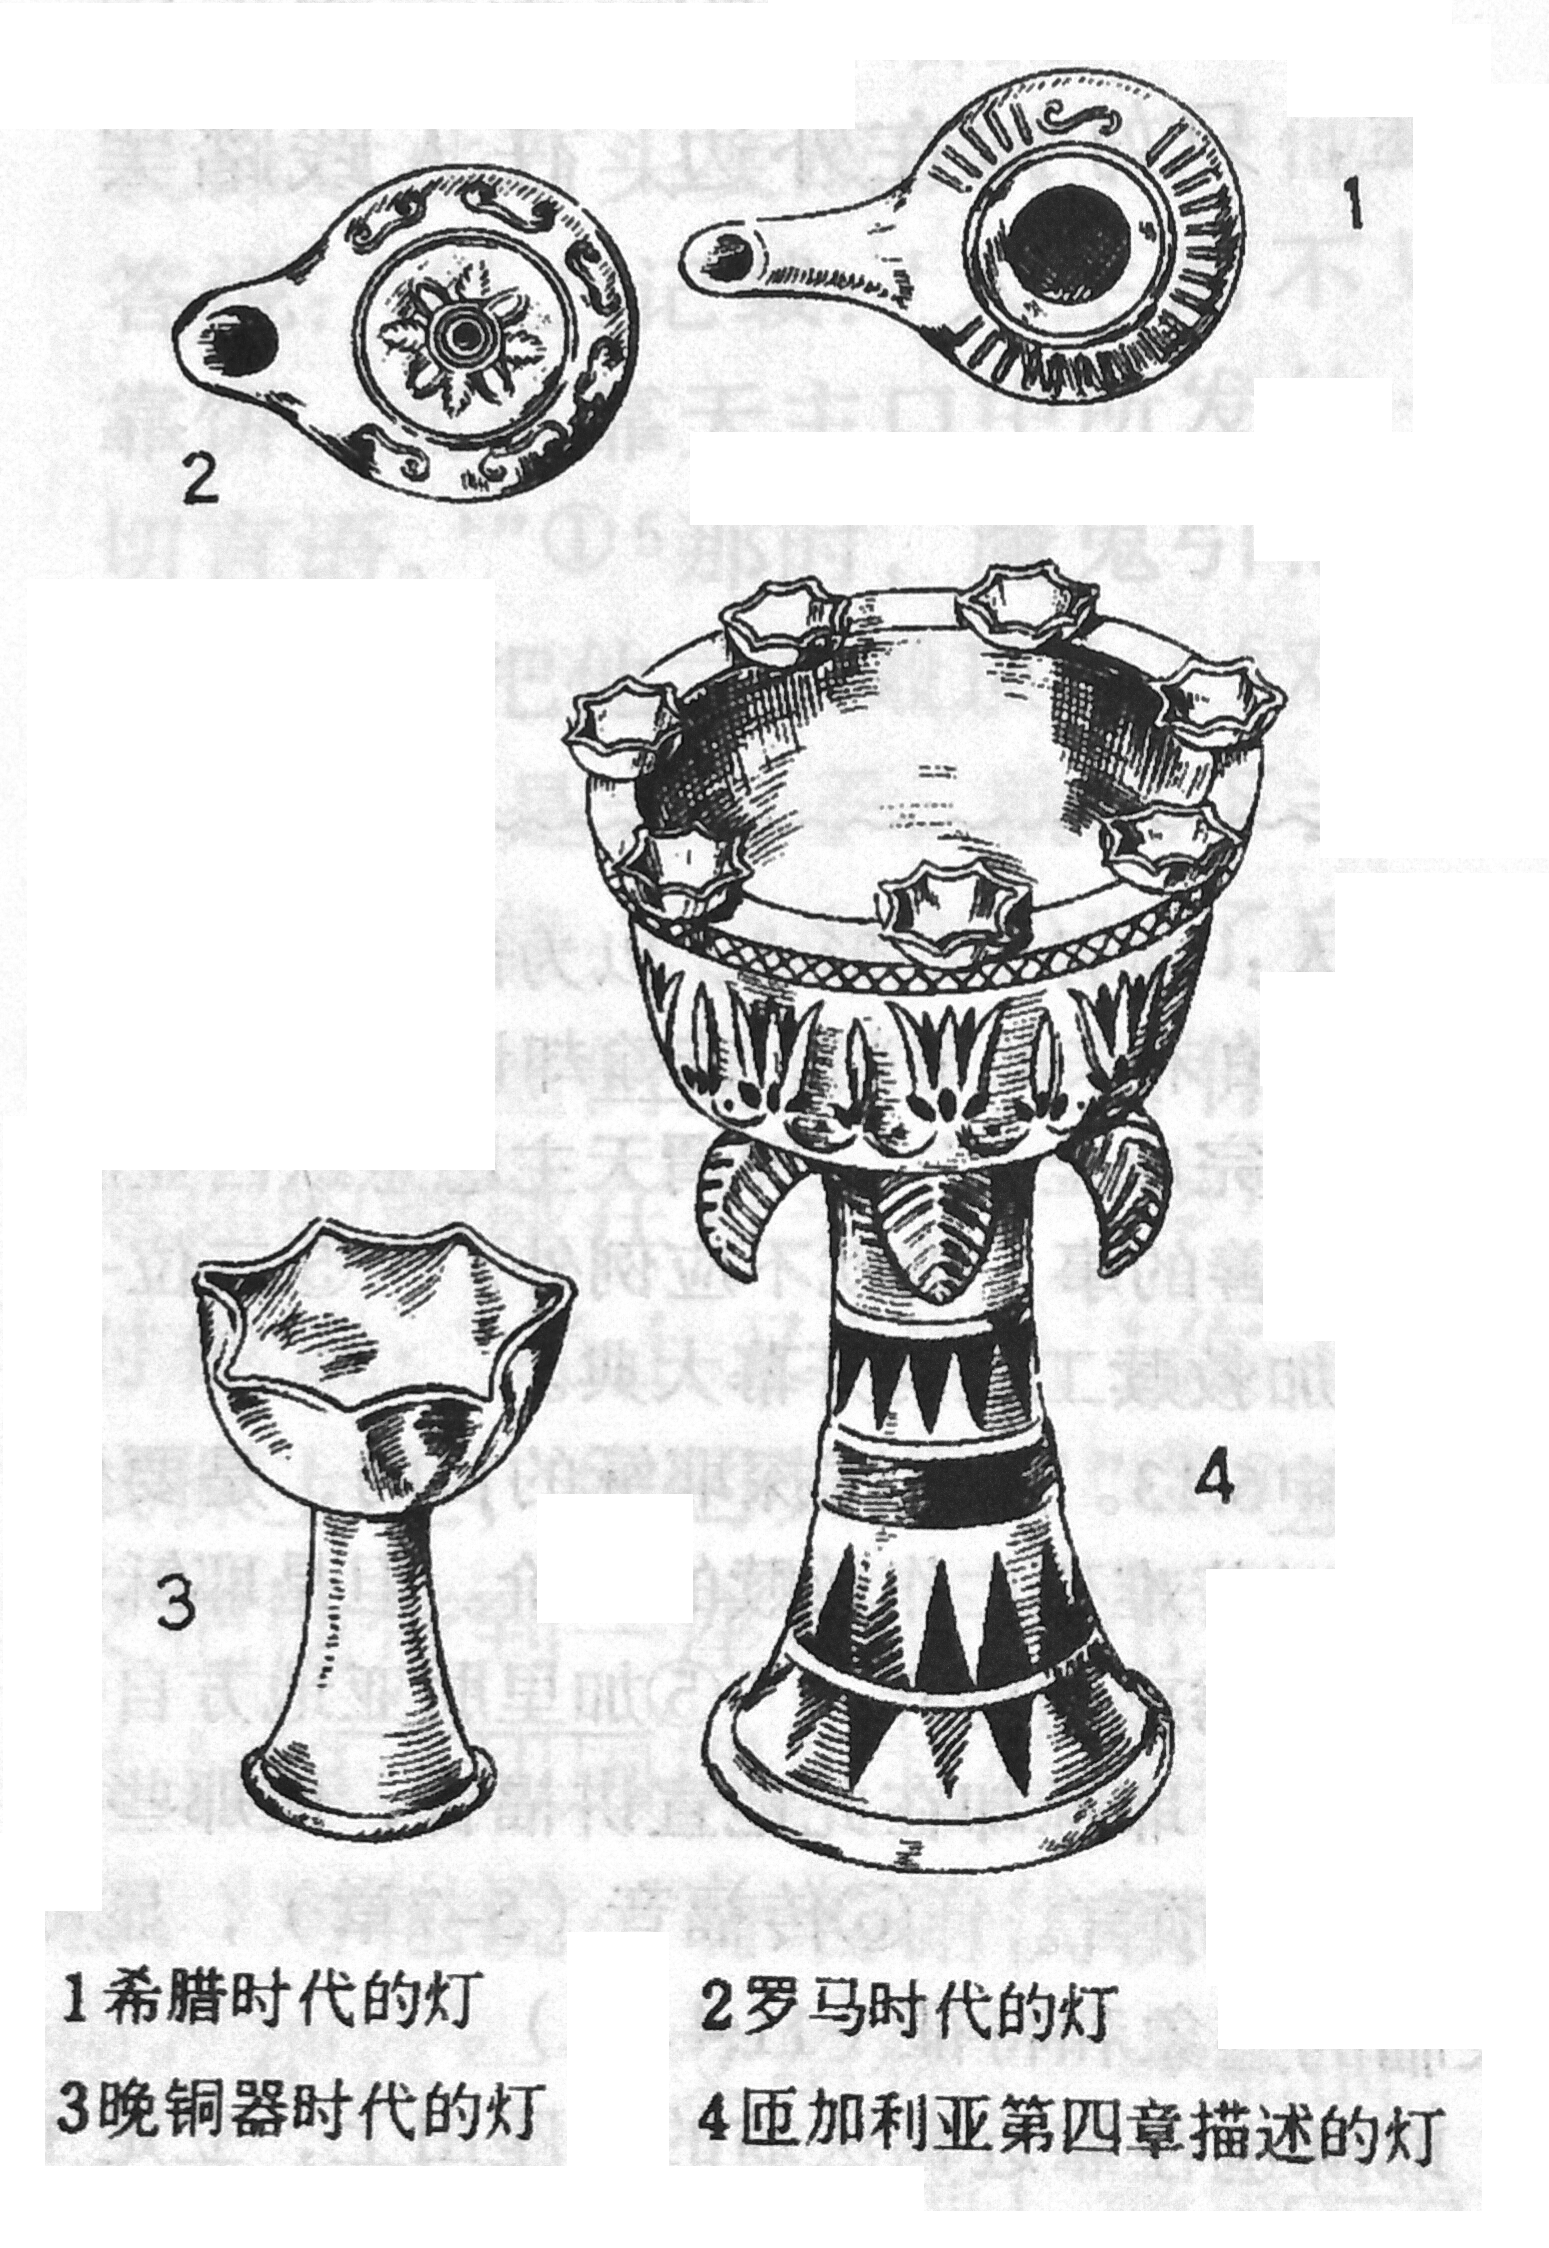
\includegraphics[width=72mm]{images/1514.png}
\end{center}


\subsubsection{新法律成全旧法律}
$^{17}$“你们不要以为我来是废除法律或先知;\textcircled{3}\NoLabelFootnote{5 \textcircled{3}法律与先知即指全部《旧约》。}我来不是为废除,而是为成全。$^{18}$我实在告诉你们:即使天地过去了,一撇或一画也决不会从法律上过去,必待一切完成。$^{19}$所以,谁若废除这些诫命中最小的一条,也这样教训人,在天国里,他将称为最小的;但谁若实行,也这样教训人,这人在天国里将称为大的。$^{20}$我告诉你们:除非你们的义德超过经师和\UL[法利塞]人的义德,你们决进不了天国。\textcircled{4}\NoLabelFootnote{5 \textcircled{4}基督徒的义德,是在于受法律的内外约束,而不是如\UL[法利塞]人所说,只在于法律的外在行为。}

$^{21}$你们一向听过给古人说:“不可杀人!”谁若杀了人,应受裁判。$^{22}$我却对你们说:凡向自己弟兄发怒的,就要受裁判;谁若向自己的弟兄说“傻子”,就要受议会的裁判;谁若说“疯子”,就要受火狱的罚。\textcircled{5}\NoLabelFootnote{5 \textcircled{5}\UL[耶稣]不但禁止人杀人,且也禁止人怀着导引人起杀机的愤怒和辱骂。“疯子”按原文是指不恭敬天主,不守法律的人。“火狱”按原文是指靠近\UL[耶路撒冷]城南烧垃圾和尸体的\UL[革厄纳]山谷(《旧约》常称\UL[本希农])。此山谷作了地狱的象征。}$^{23}$所以,你若在祭坛前,要献你的礼物时,在那里想起你的弟兄有什么怨你的事,$^{24}$就把你的礼物留在那里,留在祭坛前,先去与你的弟兄和好,然后再来献你的礼物。$^{25}$当你和你的对头还在路上,赶快与他和解,免得对头把你交与判官,判官交给差役,把你投在狱里。$^{26}$我实在告诉你:非到你还了最后的一文,决不能从那里出来。

$^{27}$你们一向听说过:“不可奸淫!”$^{28}$我却对你们说:凡注视妇女,有意贪恋她的,他已在心里奸淫了她。$^{29}$若是你的右眼使你跌倒,剜出它来,从你身上扔掉,因为丧失你一个肢体,比你全身投入地狱里,为你更好;$^{30}$若你的右手使你跌倒,砍下它来,从你身上扔掉,因为丧失你一个肢体,比你全身投入地狱里,为你更好。

$^{31}$又说过:“谁若休妻,就该给她休书。”$^{32}$我却给你们说:除了姘居外,凡休自己的妻子的,便是叫她受奸污;并且谁若娶被休的妇人,就是犯奸淫。\textcircled{6}\NoLabelFootnote{5 \textcircled{6}详见19:3-10并注。}

$^{33}$你们又一向听过对古人说:“不可发虚誓!要向上主偿还你的誓愿!”$^{34}$我却对你们说:你们总不可发誓:不可指天,因为天是天主的宝座;$^{35}$不可指地,因为地是他的脚凳;不可指\UL[耶路撒冷],因为她是大王的城市;$^{36}$也不可指你的头发誓,因为你不能使一根头发变白或变黑。$^{37}$你们的话该当是:是就说是,非就说非;其他多余的,便是出于邪恶。\textcircled{7}\NoLabelFootnote{5 \textcircled{7}17-37节,教训人守一切法律。预防犯罪,应由约束内心作起,\UL[法利塞]人即忽略了这一点。}

$^{38}$你们一向听说过:“以眼还眼,以牙还牙。”$^{39}$我却对你们说:不要抵抗恶人;而且,若有人掌击你的右颊,你把另一面也转给他。$^{40}$那愿与你争讼,拿你的内衣的,你连外衣也让给他。$^{41}$若有人强迫你走一千步,你就同他走两千步。$^{42}$求你的,就给他;愿向你借贷的,你不要拒绝。

$^{43}$你们一向听说过:“你应爱你的近人,恨你的仇人!”$^{44}$我却对你们说:你们当爱你们的仇人,当为迫害你们的人祈祷,$^{45}$好使你们成为你们在天之父的子女,因为他使太阳上升,光照恶人,也光照善人;降雨给义人,也给不义的人。$^{46}$你们若只爱那爱你们的人,你们还有什么赏报呢?税吏不是也这样作吗?$^{47}$你们若只问候你们的弟兄,你们作了什么特别的呢?外邦人不是也这样作吗?$^{48}$所以你们应当是成全的,如同你们的天父是成全的一样。”\textcircled{8}\NoLabelFootnote{5 \textcircled{8}基督徒的成全之德是爱,这爱尤其表现于爱仇人。爱仇非出于怯懦,而是效法天父恩待善人也恩待恶人的美德。}


\subsection{第六章 施舍祈祷和禁食的精神}
$^{1}$“你们应当心,不要在人前行你们的仁义,\textcircled{1}\NoLabelFootnote{6 \textcircled{1}“仁义”是泛指施舍、祈祷、禁食等善工。}为叫他们看见;若是这样,你们在天父之前,就没有赏报了。$^{2}$所以,当你施舍时,不可在你前面吹号,如同假善人在会堂及街市上所行的一样,为受人们的称赞;我实在告诉你们,他们已获得了他们他们的赏报。$^{3}$当你施舍时,不要叫你左手知道你右手所行的,$^{4}$好使你的施舍隐而不露,你父在暗中看见,必要报答你。$^{5}$当你祈祷时,不要如同假善人一样,爱在会堂及十字街头立着祈祷,为显示给人;我实在告诉你们,他们已获得了他们的赏报。\textcircled{2}\NoLabelFootnote{6 \textcircled{2}\UL[耶稣]不是指摘公众敬礼,而是指摘不由衷,只图炫耀于人的敬礼。}$^{6}$至于你,当你祈祷时,要进入你的内室,关上门,向你在暗中之父祈祷;你的父在暗中看见,必要报答你。

$^{7}$你们祈祷时,不要唠唠叨叨,如同外邦人一样,因为他们以为只要多言,便可获得垂允。$^{8}$你们不要跟他们一样,因为你们的父,在你们求他以前,已知道你们需要什么。$^{9}$所以,你们应当这样祈祷:

我们在天的父!愿你的名被尊为圣,

$^{10}$愿你的国来临,愿你的旨意承行于地,如在天上一样!

$^{11}$我们的日用粮,求你今天赐给我们;

$^{12}$宽免我们的罪债,犹如我们也宽免得罪我们的人;

$^{13}$不要让我们陷入诱惑,但救我们免于凶恶。\textcircled{3}\NoLabelFootnote{6 \textcircled{3}“天主经”是\UL[耶稣]亲自所传授的最完善的祈祷方式:前段求天主获得光荣,天国成立在世界上,世人承行主旨;后段求个人的日用急需,罪之赦,不为诱惑所陷害。参阅\uwave{路}11:2-4所载“天主经”。}

$^{14}$因为你们若宽免别人的过犯,你们的天父也必宽免你们的;$^{15}$但你们若不宽免别人的,你们的父也必不宽免你们的过犯。$^{16}$几时你们禁食,不要如同假善人一样,面带愁容;因为他们苦丧着脸,是为叫人看出他们禁食来。我实在告诉你们,他们已获得了他们的赏报。$^{17}$至于你,当你禁食时,要用油抹你的头,洗你的脸,$^{18}$不要叫人看出你禁食来,但叫你那在暗中之父看见;你的父在暗中看见,必要报答你。”


\subsubsection{归向天主的纯洁之心}
$^{19}$“你们不要在地上为自己积蓄财宝,因为在地上有虫蛀,有锈蚀,在地上也有贼挖洞偷窃;$^{20}$但该在天上为自己积蓄财宝,因为那里没有虫蛀,没有锈蚀,那里也没有贼挖洞偷窃。$^{21}$因为你的财宝在哪里,你的心也必在哪里。$^{22}$眼睛就是身体的灯。所以,你的眼睛若是康健,你的全身就都光明。$^{23}$但是,如果你的眼睛有了病,你的全身就都黑暗。那么,你身上的光明如果成了黑暗,那该是多么黑暗!”\textcircled{4}\NoLabelFootnote{6 \textcircled{4}以眼喻人心:如人心不为物欲所迷,只想望天上之事,人的生活自然合乎法度;不然,必定是非不分(\uwave{路}11:34-36)。}


\subsubsection{惟独事奉主依恃主的照顾}
$^{24}$“没有人能事奉两个主人:他或是要恨这一个而爱那一个,或是依附这一个而轻忽那一个。你们不能事奉天主而又事奉钱财。

$^{25}$为此,我告诉你们:不要为你们的生命忧虑吃什么,或喝什么;也不要为你们的身体忧虑穿什么。难道生命不是贵于食物,身体不是贵于衣服吗?$^{26}$你们仰观天空的飞鸟,它们不播种,也不收获,也不在粮仓里屯积,你们的天父还是养活它们;你们不比它们更贵重吗?$^{27}$你们中谁能运用思虑,使自己的寿数增加一肘呢?\textcircled{5}\NoLabelFootnote{6 \textcircled{5}“一肘”即言一会儿工夫。此句亦可译作:“使自己的身量增加一肘呢”。}$^{28}$关于衣服,你们又忧虑什么?你们观察一下田间的百合花怎样生长:它们既不劳作,也不纺织;$^{29}$可是我告诉你们:连\UL[撒罗满]在他极盛的荣华时代所披戴的,也不如这些花中的一朵。$^{30}$田地里的野草今天还在,明天就投在炉中,天主尚且这样装饰,信德薄弱的人那,何况你们呢?$^{31}$所以,你们不要忧虑说:我们吃什么,喝什么,穿什么?$^{32}$因为这一切都是外邦人所寻求的;你们的天父原晓得你们需要这一切。$^{33}$你们先该寻求天主的国和它的义德,这一切自会加给你们。$^{34}$所以你们不要为明天忧虑,因为明天有明天的忧虑:一天的苦足够一天受的了。”


\subsection{第七章 各种劝谕}
$^{1}$“你们不要判断人,免得你们受判断,$^{2}$因为你们用什么判断来判断,你们也要受什么判断;你们用什么尺度量给人,也要用什么尺度量给你们。$^{3}$为什么你只看见你兄弟眼中的木屑,而对自己眼中的大梁竟不理会呢?$^{4}$或者,你怎能对你的兄弟说:让我把你眼中的木屑取出来,而你眼中却有一根大梁呢?$^{5}$假善人哪!先从你眼中取出大梁,然后你才看得清楚,取出你兄弟眼中的木屑。

$^{6}$你们不要把圣物给狗,也不要把你们的珠宝投在猪前,怕它们用脚践踏了珠宝,而又转过来咬伤你们。\textcircled{1}\NoLabelFootnote{7 \textcircled{1} 圣物珠宝,指神圣的奥理,狗和猪,指心怀恶意的人。}

$^{7}$你们求,必要给你们;你们找,必要找着;你们敲,必要给你们开,$^{8}$因为凡是求的,就必得到;找的,就必找到;敲的,就必给他开。$^{9}$或者,你们中间有哪个人,儿子向他求饼,反而给他石头呢?$^{10}$或者求鱼,反而给他蛇呢?$^{11}$你们纵然不善,尚且知道把好的东西给你们的儿女,何况你们在天之父,岂不更将好的赐与求他的人?

$^{12}$所以,凡你们愿意人给你们做的,你们也要照样给人做:法律和先知即在于此。”\textcircled{2}\NoLabelFootnote{7 \textcircled{2} 旧约的总纲也不外是爱人如己。}


\subsubsection{辨别真假好坏的训言}
$^{13}$“你们要从窄门进去,因为宽门和大路导入丧亡;但有许多的人从那里进去。$^{14}$那导人生命的门是多么窄,路是多么狭!找到它的人的确不多。\textcircled{3}\NoLabelFootnote{7 \textcircled{3} 窄门狭路指守诫命,背十字架的生活。}

$^{15}$你们要提防假先知!他们来到你们跟前,外披羊毛,内里却是凶残的豺狼。$^{16}$你们可凭他们的果实辨别他们:荆棘上岂能收到葡萄?或者蒺藜上岂能收到无花果?$^{17}$这样,凡是好树都结好果子,而坏树都结坏果子;$^{18}$好树不能结坏果子,坏树也不能结好果子。$^{19}$凡不结好果子的树,必要砍倒,投入火中。$^{20}$所以,你们可凭他们的果实辨别他们。

$^{21}$不是凡向我们“主啊!主啊!”的人,就能进天国;而是那承行我在天之父旨意的人,才能进天国。$^{22}$到那一天有许多人要向我说:主啊!主啊!我们不是因你的名字说过预言,因你的名字驱过魔鬼,因你的名字行过许多奇迹吗?$^{23}$那时,我必要向他们声明说:我从来不认识你们,你们这些作恶的人,离开我吧!”


\subsubsection{山中圣训的结论}
${24}$“所以,凡听了我这些话而实行的,就好像一个聪明人,把自己的房屋建在磐石上:${25}$雨淋,水冲,风吹,袭击那座房屋,它并不坍塌,因为基础是建在磐石上。${26}$凡听了我这些话而不实行的,就好像一个愚昧人,把自己的房屋建在沙土上:${27}$雨淋,水冲,风吹,袭击那座房屋,它就坍塌了,且坍塌的很惨。”

${28}$\UL{耶稣}讲完了这些话,群众都惊奇他的教训,${29}$因为他教训他们,正像有权威的人,不像他们他们的经师。


\section{建立天国的准备 耶稣行的奇迹}


\subsection{第八章 治好癞病人}
${1}$\UL{耶稣}从山上下来,有这么多群众跟随他。${2}$看,有一个癞病人前来叩拜\UL{耶稣}说:“主!你若愿意,就能洁净我。”${3}$\UL{耶稣}就伸手抚摸他说:“我愿意,你洁净了吧!”他的癞病立刻就洁净了。${4}$\UL{耶稣}对他说:“小心,不要对任何人说!但去叫司祭检验你,献上\UL{梅瑟}所规定的礼物,给他们当做证据。”\textcircled{1}\NoLabelFootnote{8 \textcircled{1} 圣史记述\UL{耶稣}为天国的立法者与导师之后(5-7章),即记述\UL{耶稣}所显的奇迹(8-9章),证明他的全能。按\uwave{肋}14,痊愈的癞病人经司祭检验献祭后,方准与人来往。\UL{耶稣}吩咐癞病人如此做,是叫司祭界知道他处处守法律。}


\subsubsection{治好百夫长的仆人}${5}$\UL{耶稣}进了\UL{葛法翁},有一位百夫长来到他跟前,求他${6}$说:“主!我的仆人瘫痪了,躺在家里,疼痛的狠厉害。”${7}$\UL{耶稣}对他说:“我去治好他。”${8}$百夫长答说:“主!我不堪当你到舍下来,你只要说一句话,我的仆人就会好的。${9}$因为我虽是属人权下的人,但是我也有士兵属我权下;我对这个说:你去,他就去;对另一个说:你来,他就来;对我的奴仆说:你作这个,他就作。”${10}$\UL{耶稣}听了,非常诧异,就对跟随的人说:“我实在告诉你们:在\UL{以色列}我从未遇见过一个人,有这样大的信心。${11}$我给你们说:将有许多人从东方和西方来,同\UL{亚巴郎}、\UL{依撒格}和\UL{雅各伯}在天国里一起坐席;${12}$本国的子民,反要被驱逐到外边黑暗里;那里要有哀号和切齿。”${13}$\UL{耶稣}遂对百夫长说:“你回去,就照你所信的,给你成就吧!”仆人就在那时刻痊愈了。\textcircled{2}\NoLabelFootnote{8 \textcircled{2} 外教的百夫长因谦逊和信德寻到了与圣祖赴天国圣宴的路,自夸为\UL{亚巴郎}子孙的\UL{法利塞}人却自入迷途,被拒于天国门外。}


\subsubsection{在伯多禄家中治好病人}
${14}$\UL{耶稣}来到\UL{伯多禄}家里,看见\UL{伯多禄}的岳母躺着发烧,${15}$就摸了她的手,热症就从她身上退了。她便起来伺候他。${16}$到了晚上,人们给他送来了许多附魔的人,他一句话就驱逐了恶神;治好了一切有病的人。${17}$这样,就应验了那藉\UL{依撒意亚}先知所说的话:“他承受我们的脆弱,担荷了我们的疾病。”\textcircled{3}\NoLabelFootnote{8 \textcircled{3} \uwave{依}53:4。}


\subsubsection{跟随耶稣的条件}
${18}$\UL{耶稣}看见许多群众围着自己,就吩咐往外岸去。${19}$有一位经师前来,对他说:“师傅,你不论往哪里去,我要跟随你。”${20}$\UL{耶稣}给他说:“狐狸有穴,天上的飞鸟有巢,但是人子却没有枕头的地方。”${21}$门徒中有一个对他说:“主,请许我先去埋葬我的父亲。”${22}$\UL{耶稣}对他说:“你跟随我吧!任凭死人去埋葬他们的死人!”\textcircled{4}\NoLabelFootnote{8 \textcircled{4} \UL{耶稣}常自称“人子”,表示他负有默西亚的使命(\uwave{达}7:13、14)。心志不坚,恋念骨肉的人,不宜做\UL{耶稣}的门徒,因为跟随\UL{耶稣}宣传天国的人,须有慷慨就义的精神(\uwave{路}9:57-62)}


\subsubsection{平息风浪}
${23}$\UL{耶稣}上了船,他的门徒跟随着他。${24}$忽然海里起了大震荡,以致那船为浪所掩盖,\UL{耶稣}却睡着了。${25}$他们遂前来唤醒他说:“主!救命啊!我们要丧亡了。”${26}$\UL{耶稣}对他们说:“小信德的人啊!你们为什么胆怯?”就起来叱责风和海,遂大为平静。${27}$那些人惊讶说:“这是怎样怎样的一个人呢?竟连风和海也听从他!”


\subsubsection{医好革辣撒两个附魔的人}
${28}$\UL{耶稣}来到对岸\UL{加达辣}人的地方,有两个附魔的人从坟墓里走出,向他走来;他们异常凶猛,以致没有人能从那条路上经过。${29}$他们喊说:“天主子,我们与你有什么相干?时期还没有到,你就来这里苦害我们吗?”${30}$离他们很远,有一大群猪正在牧放。${31}$魔鬼恳求\UL{耶稣}说:“你若驱逐我们,就赶我们进入猪群吧!”${32}$\UL{耶稣}对他们说:“去吧!”魔鬼就出来进入猪内;忽然全群猪从山崖上直冲入海,死在水里。${33}$放猪的便逃走,来到城里,把这一切和附魔人的事都报告了。${34}$全城的人就出来见\UL{耶稣},一见了他,就求他离开他们他们的境界。\textcircled{5}\NoLabelFootnote{8 \textcircled{5} \uwave{谷}5:1-20;\uwave{路}8:26-39叙述治好附魔的人较详。\UL{加达辣}按\uwave{谷}作\UL{革辣撒},\UL{革辣撒}为\UL{加达辣}地方的乡村。这地方的人为外教人,见\UL{耶稣}治好了两个附魔的人,理应收留耶稣;但他们不知重视此事,只以损失财物为重。}


\subsection{第九章 治好瘫子}
${1}$\UL{耶稣}上船过海,来到了自己的城。\textcircled{1}\NoLabelFootnote{9 \textcircled{1} “自己的城”,即指\UL{葛法翁},是\UL{耶稣}在\UL{加里肋亚}省传教的中心。}${2}$看,有人给他送来一个躺在床上的瘫子,\UL{耶稣}一见他们的信心,就对瘫子说:“孩子,你放心!你的罪赦了。”${3}$经师中有几个人心里说:“这人说了亵渎的话。”${4}$\UL{耶稣}看透他们的心意,说:“你们为什么心里思念恶事呢?${5}$什么比较容易呢?是说:你的罪赦了,或是说:起来行走吧?${6}$为叫你们知道,人子在地上有赦罪的权柄——就对瘫子说:起来,拿起你的床,回家去吧!”${7}$“那人就起来,回家去了。”${8}$群众见了,就都害怕起来,遂归光荣于天主,因他赐给了人们这样大的权柄。\textcircled{2}\NoLabelFootnote{9 \textcircled{2} 此二者都必须有天主的能力才能办到:若\UL{耶稣}仅一句话就治好那人的病,证明他自然也能赦他的罪。}


\subsubsection{玛窦被召为徒}
${9}$\UL{耶稣}从那里前行,看见一个人在税关那里坐着,名叫\UL{玛窦},对他说:“跟随我!”他就起来跟随了\UL{耶稣}.${10}$当\UL{耶稣}在屋里坐席时,有许多税吏和罪人也来同\UL{耶稣}和他的门徒一起坐席。${11}$\UL{法利塞}人看见,就对他的门徒说:“你们的老师为什么同税吏和罪人一起进食呢?”${12}$\UL{耶稣}听见了,就说:“不是健康健康的人需要医生,而是有病的人。${13}$你们去研究一下:‘我喜欢仁爱胜过祭献’是什么意思;我不是来召义人,而是来召罪人。”\textcircled{3}\NoLabelFootnote{9 \textcircled{3} \uwave{欧}6:6。义人,在此是指只以守法律自以为成义,而不接受\UL{耶稣}宣讲的人。}


\subsubsection{禁食问题的冲突}
${14}$那时,\UL{若翰}的门徒来到他跟前说:“为什么我们和\UL{法利塞}人多次禁食,而你的门徒却不禁食呢?”${15}$\UL{耶稣}对他们说:“伴郎岂能当新郎与他们在一起的时候悲哀?\textcircled{4}\NoLabelFootnote{9 \textcircled{4} 按\UL{犹太}人婚宴,为期共八天;在此八天内若遇禁食之日,亦不禁食。\UL{耶稣}在世是与新娘(教会)结婚的时期,因此自比为新郎,以宗徒为伴郎。}但日子将要来到:当新郎从他们他们中被劫去时,那时他们就要禁食了。${16}$没有人用未漂过的布作补丁,补在旧衣服上的,因为补上的必扯裂了旧衣,破绽就更加坏了。${17}$也没有人把新酒装入旧皮囊里的;不然,皮囊一破裂,酒也流了,皮囊也坏了;而是应把新酒装在新皮囊里,两样就都得保全。”\textcircled{5}\NoLabelFootnote{9 \textcircled{5} 旧衣与旧囊指\UL{法利塞}人所固守的惯例和制度;新布和新酒指福音的精神。此处经文大旨是:福音的精神不易为旧约宗教的人所容纳。}


\subsubsection{治好患血漏的妇人复活雅依洛的女儿}
${18}$\UL{耶稣}向他们说这话的时候,有一位首长前来跪拜他说:“我的女儿刚才死了,可是请你来,把你的手放在她身上,她必会活。”${19}$\UL{耶稣}起来跟他去了;他的门徒也跟了去。${20}$看,有一个患血漏十二年的女人,从后面走近,摸了他的衣服穗头,${21}$因为她心里想:“只要我一摸他的衣服,我就会好了。”${22}$\UL{耶稣}转过身来,看着她说“女儿,放心吧!你的信德救了你。”从那时起,那女人就好了。${23}$\UL{耶稣}来到首长家里,看见吹笛的和乱哄哄的群众,${24}$就说:“你们走开吧!女孩子没有死,只是睡着了。”他们都讥笑他。${25}$把群众赶出去以后,\UL{耶稣}就进去,拿起女孩子的手,小女孩就起来了。${26}$这消息传遍了那整个地区。


\subsubsection{使两个瞎子复明}
${27}$\UL{耶稣}从那里前行,有两个瞎子跟着他喊说:“\UL{达味}之子!可怜我们吧!”\textcircled{6}\NoLabelFootnote{9 \textcircled{6} “\UL{达味}之子”为默西亚另一名称(12:23,21:9)。}${28}$他一来到家,瞎子便走到他跟前;\UL{耶稣}对他们说:“你们信我能作这事吗?”他们对他说:“是,主!”${29}$于是\UL{耶稣}摸他们他们的眼说:“照你们的信德,给你们成就吧!”${30}$他们的眼开了。\UL{耶稣}严厉警戒他们说:“你们当心,不要使任何人知道。”${31}$但他们出去,就在那整个地区把他传扬开了。


\subsubsection{治好附魔的哑巴}
${32}$他们出去后,看,有人给\UL{耶稣}送来一个附魔的哑巴。${33}$魔鬼一被赶出去,哑巴就说出话来。群众惊奇说:“在\UL{以色列}从未出现过这样的事情。”${34}$但\UL{法利塞}人们却说:“他是仗赖魔王驱魔。”


\subsubsection{庄稼多工人少}
${35}$\UL{耶稣}周游各城各村,在他们的会堂内施教,宣讲天国的福音,治好一切疾病。一切灾殃。${36}$他一见到群众,就对他们动了慈心,因为他们困苦流离,像没有牧人的羊。${37}$于是对自己的门徒说:“庄稼固多,工人却少,${38}$所以你们应当求庄稼的主人派遣工人,来收他的庄稼。”


\section{教导宗徒传教}


\subsection{第十章 首次派遣十二宗徒传教}
${1}$\UL{耶稣}将他的十二门徒叫来,授给他们制伏邪魔的权柄,可以驱逐邪魔,医治各种病症,各种疾苦。${2}$这是十二宗徒的名字:第一个是称为\UL{伯多禄}的\UL{西满},和他的兄弟\UL{安德肋},\UL{载伯德}的儿子\UL{雅各伯}和他的弟弟\UL{若望},${3}$\UL{斐理伯}和\UL{巴尔多禄茂},\UL{多默}和税吏\UL{玛窦},\UL{阿耳斐}的儿子\UL{雅各伯}和\UL{达陡},${4}$热诚者\UL{西满}和负卖\UL{耶稣}的\UL{犹达斯}\UL{依斯加略}。${5}$\UL{耶稣}派遣这十二人,嘱咐他们说:“外邦人的路,你们不要走;\UL{撒玛黎雅}人的城,你们不要进,${6}$你们宁可往\UL{以色列}家迷失了的羊那里去。${7}$你们在路上应宣讲说:天国临近了。\textcircled{1}\NoLabelFootnote{10 \textcircled{1} 按选已十二支派的数目,耶稣选了十二“宗徒”(或称“使徒”),作为“新\UL{以色列}”选民——圣教会的宗师。当时,他打发他们,要他们只给\UL{以色列}家“迷失了的羊”宣讲福音,因为\UL{以}民是天主的选民,有听受福音的优先权。\UL{耶稣}升天时才命令宗徒去外邦传教。}${8}$病人,你们要治好;死人,你们要复活;癞病人,你们要洁净;魔鬼,你们要驱逐;你们白白得来的,也要白白分施。


${9}$你们不要在腰带里备下金、银、铜钱;${10}$路上不要带口袋,也不要带两件内衣,也不要穿鞋,也不要带棍杖,因为工人自当有他的食物。\textcircled{2}\NoLabelFootnote{10 \textcircled{2} \UL{耶稣}教训传福音的不依仗金钱财物,而应依仗福音本身的德能。为天主工作的人,天主自会照料他。}${11}$你们不论进了哪一城或哪一村,查问其中谁是当得起的,就住在那里,直到你们离去。${12}$你们进那一家时,要向它请安。${13}$倘若这一家是堪当的,你们的平安就必降临到这一家;倘若是不堪当的,你们的平安仍归于你们。${14}$谁若不接待你们,也不听你们你们的话,当你们从那一家或那一城出来时,应把尘土由你们的脚上拂去。\textcircled{3}\NoLabelFootnote{10 \textcircled{3} “拂土”是经师教训\UL{犹太}人由外邦进入圣地前所应行的一种象征行为,表示自己与敬拜邪神的人完全断绝关系。此处是以不接受福音的\UL{犹太}人与外邦人相比。}${15}$我实在告诉你们:在审判的日子,\UL{索多玛}和\UL{哈摩辣}地所受的惩罚,比那座城所受的还要轻。


${16}$看,我派遣你们好像羊进入狼群中,所以你们要机警如同蛇,纯朴如同鸽子。${17}$你们要提防世人,因为他们要把你们交给公议会,要在他们的会堂里鞭打你们;${18}$并且你们要为我的缘故,被带到总督和君王前,对他们和外邦人作证。


${19}$当人把你们交出时,你们不要思虑:怎么说,或说什么,因为在那时刻,自会赐给你们应说什么。${20}$因为说话的不是你们,而是你们父的圣神在你们内说话。


${21}$兄弟要将兄弟,父亲要将儿子置于死地,儿女也要起来反对父母,要将他们害死。\textcircled{4}\NoLabelFootnote{10 \textcircled{4} 不是\UL{耶稣}愿意至亲不和,而是他的福音作了“反对的记号”(\uwave{路}2:24),因为不信的要反对那信了的(35节)。}${22}$你们为了我的名字,要为众人所恼恨;唯独坚持到底的,才可得救。${23}$但是,几时人们在这城迫害你们,你们就逃往另一城去;我实在告诉你们:直到人子来时,你们还未走完\UL{以色列}的城邑。\textcircled{5}\NoLabelFootnote{10 \textcircled{5} 23节是指迫害教会的事,都十分短暂,不足害怕,而胜利常属于耶稣。}


${24}$没有徒弟胜过师傅的,也没有仆人胜过他主人的;${25}$徒弟能如他的师傅一样,仆人能如他的主人一样,也就够了。若人们称家主为“贝耳则步”,\textcircled{6}\NoLabelFootnote{10 \textcircled{6} “贝耳则步”本为\UL{培肋}\UL{舍肋}人神祇的名字,后转为魔王的称呼(12:24)。}对他的家人更该怎样呢?${26}$所以,你们不要害怕他们;因为没有遮掩的事,将来不被揭露的;也没有隐藏的事,将来不被知道的。${27}$我在暗中给你们所说的,你们要在光天化日之下报告出来;你们由耳语所听到的,要在屋顶上张扬出来。${28}$你们不要害怕那杀害肉身,而不能杀害灵魂的;但更要害怕那能使灵魂和肉身陷于地狱中的。${29}$两只麻雀不是卖一个铜钱吗?但若没有你们天父的许可,它们中连一只也不会掉在地上。${30}$就是你们的头发,也都一一数过了。${31}$所以,你们不要害怕;你们比许多麻雀还贵重呢!${32}$凡在人前承认我的,我在我天上的父前也必承认他;${33}$但谁若在人前否认我,我在我天上的父前也必否认他。


${34}$你们不要以为我来,是为把平安带到地上;我来不是为带平安,而是带刀剑,\textcircled{7}\NoLabelFootnote{10 \textcircled{7} 刀剑的比喻是指因\UL{耶稣}的福音而引起的不睦。}${35}$因为我来,是为叫人脱离自己的父亲,女儿脱离自己的母亲,儿媳脱离自己的婆母;${36}$所以,人的仇敌,就是自己的家人。${37}$谁爱父亲或母亲超过我,不配是我的;谁爱儿子或女儿超过我,不配是我的。${38}$谁不背起自己的十字架跟随我,不配是我的。


${39}$谁获得自己的性命,必要丧失性命;谁为我的缘故,丧失了自己的性命,必要获得性命。${40}$谁接纳你们,就是接纳我;谁接纳我,就是接纳那派遣我来的。${41}$谁接纳一位先知,因他是先知,将领受先知的赏报;谁接纳一位义人,因他是义人,将领受义人的赏报。${42}$谁若只给这些小子中的一个,一杯凉水喝,因他是门徒,我实在告诉你们,他决失不了他的赏报。”


\section{天国的奥秘}


\subsection{第十一章 若翰遣徒访问耶稣}
${1}$\UL{耶稣}嘱咐完了他的十二门徒,就从那里走了,为在他们他们的城里施教宣讲。

${2}$\UL{若翰}在狱中听到了\UL{基督}所行的,就派遣他的门徒去,${3}$对他说:“你就是要来的那一位,或是我们还要等候另一位?”${4}$\UL{耶稣}回答他们说:“你们去,把你们所见所闻的报告给\UL{若翰}:${5}$瞎子看见,瘸子行走,癞病人得了洁净,聋子听见,死人复活,穷苦人得了喜讯。${6}$凡不因我而绊倒的,是有福的!”\textcircled{1}\NoLabelFootnote{11 \textcircled{1} \UL{耶稣}仅以\uwave{依}29:18、19,35:5、6,61:1对默西亚的预言贴在自己身上,答复\UL{若翰}的询问。“绊倒”即谓因怀疑不信而致丧亡之意。}


\subsubsection{耶稣称赞若翰}
${7}$他们走后,\UL{耶稣}就对群众论\UL{若翰}说:“你们出去到荒野里,是为看什么呢?为看风摇曳的芦苇吗?${8}$你们出去到底是为看什么?为看一位穿细软衣服的人吗?啊!那穿细软衣服的人是在王宫里。${9}$你们究竟为什么出去?为看一位先知吗?是的!我给你们说:而且他比先知还大。${10}$关于这人,经上记载说:“看,我派遣我的使者在你面前,他要在你前面预备你的道路。”\textcircled{2}\NoLabelFootnote{11 \textcircled{2} \uwave{拉}3:1。}${11}$我实在告诉你们:在妇女所生者中,没有兴起一位比洗者\UL{若翰}更大的;但在天国里最小的,也比他大。\textcircled{3}\NoLabelFootnote{11 \textcircled{3} 论\UL{若翰}作前驱的职位,没有能超过他的;但论他所享的福分,远不及新约的子民(\uwave{路}7:24、25),因为他还是属于旧约的人。}${12}$由洗者\UL{若翰}的日子直到如今,天国是以猛力夺取的,以猛力夺取的人,就攫取了它,${13}$因为众先知和法律讲说预言,直到\UL{若翰}为止。${14}$若是你们愿意接受,他就是那位要来的\UL{厄里亚}。\textcircled{4}\NoLabelFootnote{11 \textcircled{4} 按当时的传说(17:10-12;\uwave{拉}3:23),默西亚来临时\UL{厄里亚}应先来。\UL{耶稣}称\UL{若翰}为\UL{厄里亚},不是说他真是\UL{厄里亚},而是说他具有\UL{厄里亚}的精神(\uwave{路}1:17)。}${15}$有耳的,听吧!”


\subsubsection{责斥同代的人}
${16}$“我可把这一代比作什么呢?它像坐在大街上的儿童,向其他的孩子喊叫,${17}$说:我们给你们吹了笛,你们却不跳舞;我们唱了哀歌,你们却不捶胸。${18}$\UL{若翰}来了,也不吃,也不喝,他们便说:他附了魔;${19}$人子来了,也吃也喝,他们却说:看哪!一个贪吃嗜酒的人,税吏和罪人的朋友!但智慧必藉自己的工程彰显自己的正义。\textcircled{5}\NoLabelFootnote{11 \textcircled{5} 不拘\UL{犹太}人怎样无理取闹,执迷不悟,但天主救世的计划必藉着有真知灼见的人(\UL{耶稣}、\UL{若翰}、有信德的小民)彰显于外。}”

${20}$那时,\UL{耶稣}就开始谴责那曾看过他许多异能的城邑,因为她们没有悔改:${21}$“\UL{苛辣匝因},你是有祸的!\UL{贝特赛达},你是有祸的!因为在你们那里所行的异能,如果行在\UL{提洛}和\UL{漆冬},她们早已身披苦衣,头上撒灰做补赎了。${22}$但是我给你们说:在审判的日子,\UL{提洛}和\UL{漆冬}所受的惩罚也要比你们容易忍受。${23}$还有你,\UL{葛法翁}!莫非你要被高举到天上吗?将来你必下到阴府里;因为在你那里所行的异能,如果行在\UL{索多玛},她必会存留到今天。${24}$但是我给你们说:在审判的日子,\UL{索多玛}地所受的惩罚也要比你们容易忍受。”


\subsubsection{诚实人获得喜讯}
${25}$就在那时候,\UL{耶稣}发言说:“父啊!天地的主宰!我称谢你,因为你将这些事瞒住了智慧和明达的人。而启示给小孩子。\textcircled{6}\NoLabelFootnote{11 \textcircled{6} “智慧和明达的人”,指自以为智慧明达的\UL{法利塞}人;“小孩子”指自认无能的诚实谦卑的门徒。}${26}$是的,父啊!你原来喜欢这样。${27}$我父将一切交给了我;除了父外,没有人认识子;除了子和子所愿意启示的人外,也没有人认识父。

${28}$凡劳苦和负重担的,你们都到我跟前来,我要使你们安息。${29}$你们背起我的轭,跟我学吧!因为我是良善心谦的:这样你们必要找得你们灵魂的安息,${30}$因为我的轭是柔和的,我的担子是轻松的。”